\section{Monalisa}
First, the image is read using \texttt{matplotlib}'s \texttt{imread()} method.
Then we run a for loop for the shift amount and use \texttt{numpy}'s slicing to shift the image.
After, the shifted image is obtained, it's correlation with the original image is calculated using \texttt{numpy}'s \texttt{corrcoef()} method.
The shift amount is stored in \texttt{correlations\_x} and the correlation value is stored in \texttt{correlations\_y}.
Finally, a plot is made using \texttt{matplotlib}'s \texttt{plot()} method.

\begin{figure}[H]
	\centering
	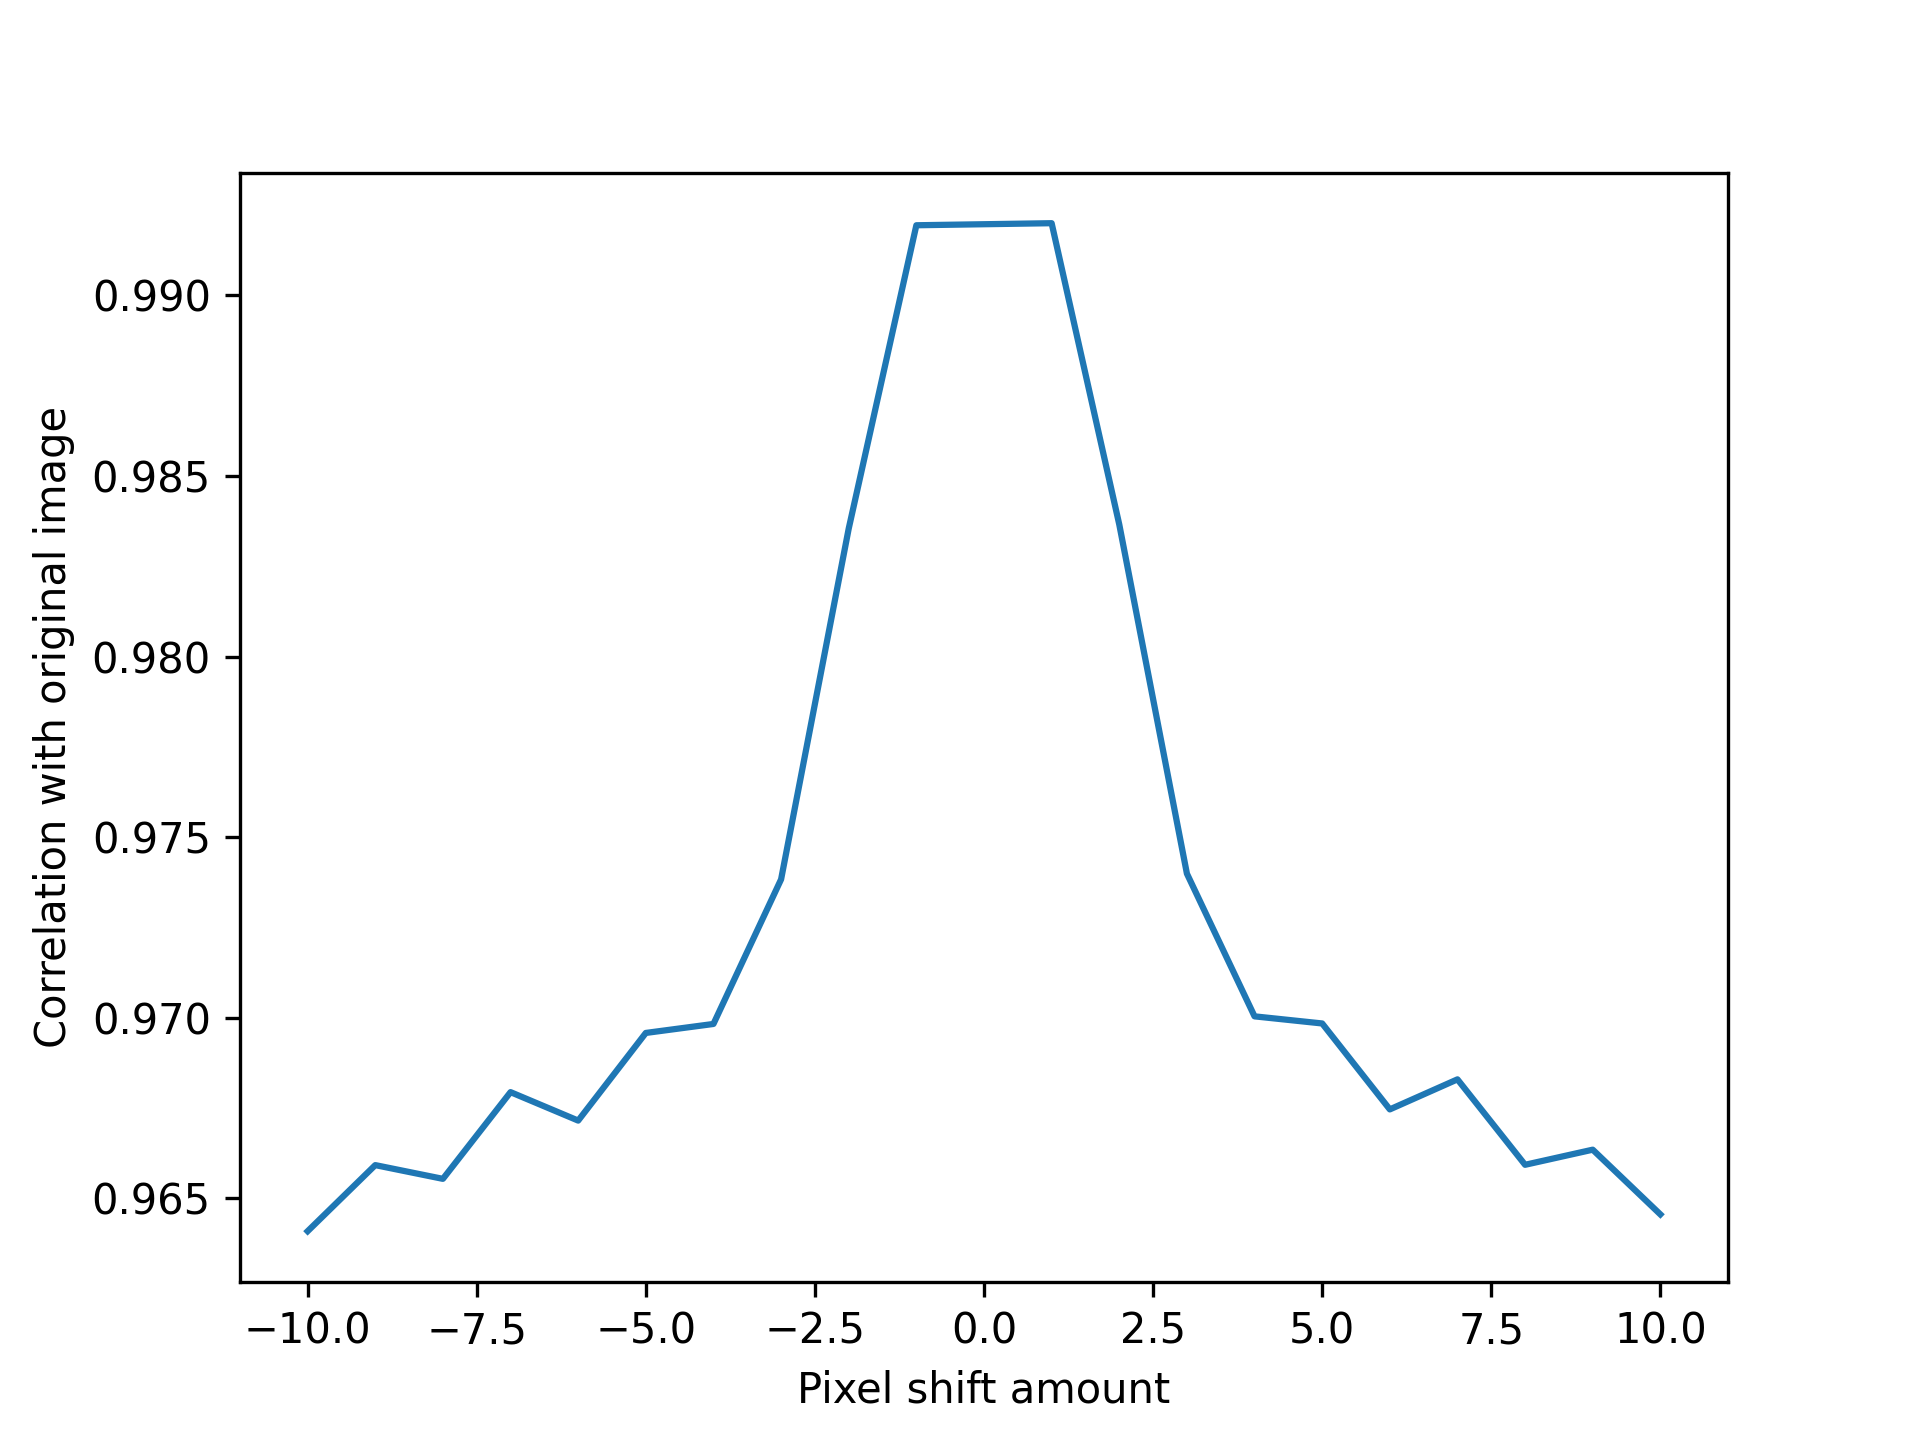
\includegraphics[width=0.8\textwidth]{img/correlation.png}
	\caption{Plot of correlation values against the pixel shift amounts}
	\label{fig:correlation}
\end{figure}

\begin{lstlisting}[language=Python, caption={Python code to compute and plot the correlations of the shifted images}, label=lst:correlation]
# imports
import numpy as np
import matplotlib.pyplot as plt

plt.rcParams["figure.dpi"] = 300  # higher resolution output images

img = plt.imread("Mona_Lisa.jpg")  # read the image

plt.imshow(img)
plt.gca().set_xlabel("x")  # set the x-label of the current Axes (returned by the gca)
plt.gca().set_ylabel("y")  # set the y-label of the current Axes

correlations_x = np.array(
    list(range(-10, 0)) + list(range(1, 11))
)  # x axis values for correlation plot
correlations_y = np.zeros(20)  # y axis values for correlation plot

for k in range(20):
    tx = correlations_x[k]  # shift amount
    img_new = np.zeros_like(img, dtype=np.uint8)  # create a new image
    if tx >= 0:
        img_new[:, tx:] = img[:, : img.shape[1] - tx]
    else:
        img_new[:, : img.shape[1] + tx] = img[:, -tx:]
    correlations_y[k] = np.corrcoef(img.flatten(), img_new.flatten())[
        0, 1
    ]  # store correlation

# plot the correlations
plt.figure()
plt.plot(correlations_x, correlations_y)
plt.xlabel("Pixel shift amount")
plt.ylabel("Correlation with original image")
plt.savefig("correlation.png")
\end{lstlisting}

The plot obtained is shown in \Cref{fig:correlation}.
We can see that the correlation between the original image and the shifted image decreases as the shift amount increases.
This is because adjacent pixels in the image have higher correlation as compared to pixels that are apart. In high resolution images, colors transition smoothly (without an abrupt change) between adjacent pixels.
This is easy to observe from \Cref{fig:shifted_images}.


\begin{figure}[H]
	\centering
	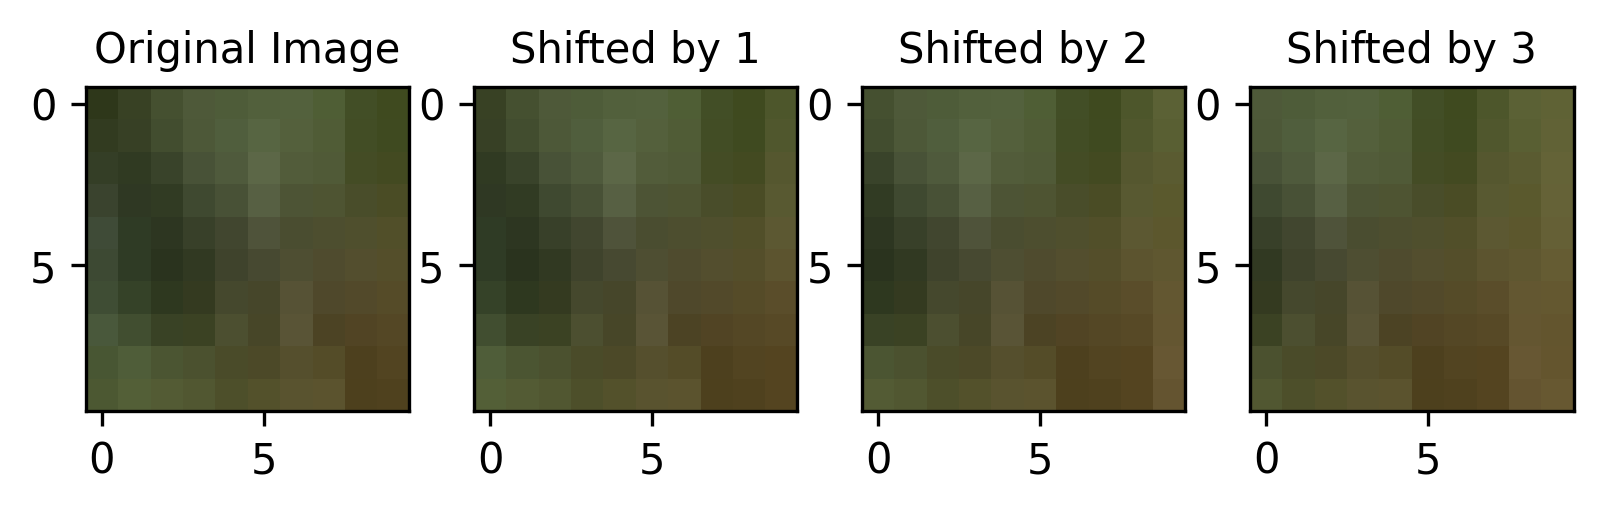
\includegraphics{img/shifted_images.png}
	\caption{Top left 10x10 pixels of the original and shifted images}
	\label{fig:shifted_images}
\end{figure}

To obtain the histogram of the image, we first convert the image to grayscale to get pixel intensities.
This is done using the formula
\[I = 0.2989 \times R + 0.5870 \times G + 0.1140 \times B\]
Then we use two for loops to iterate over all the pixels in the image, and calculate the histogram (frequency of each pixel intensity), which is stoed in variable \texttt{h}.
The histogram is then normalised by dividing by the total number of pixels in the image, this is soted in the variable \texttt{p}.
Finally, the histogram is plotted using \texttt{matplotlib}'s \texttt{hist()} method, but by using the \texttt{weights} parameter as we've already computed the histogram.
The output is shown in \Cref{fig:normalized_histogram}.

\begin{figure}[H]
	\centering
	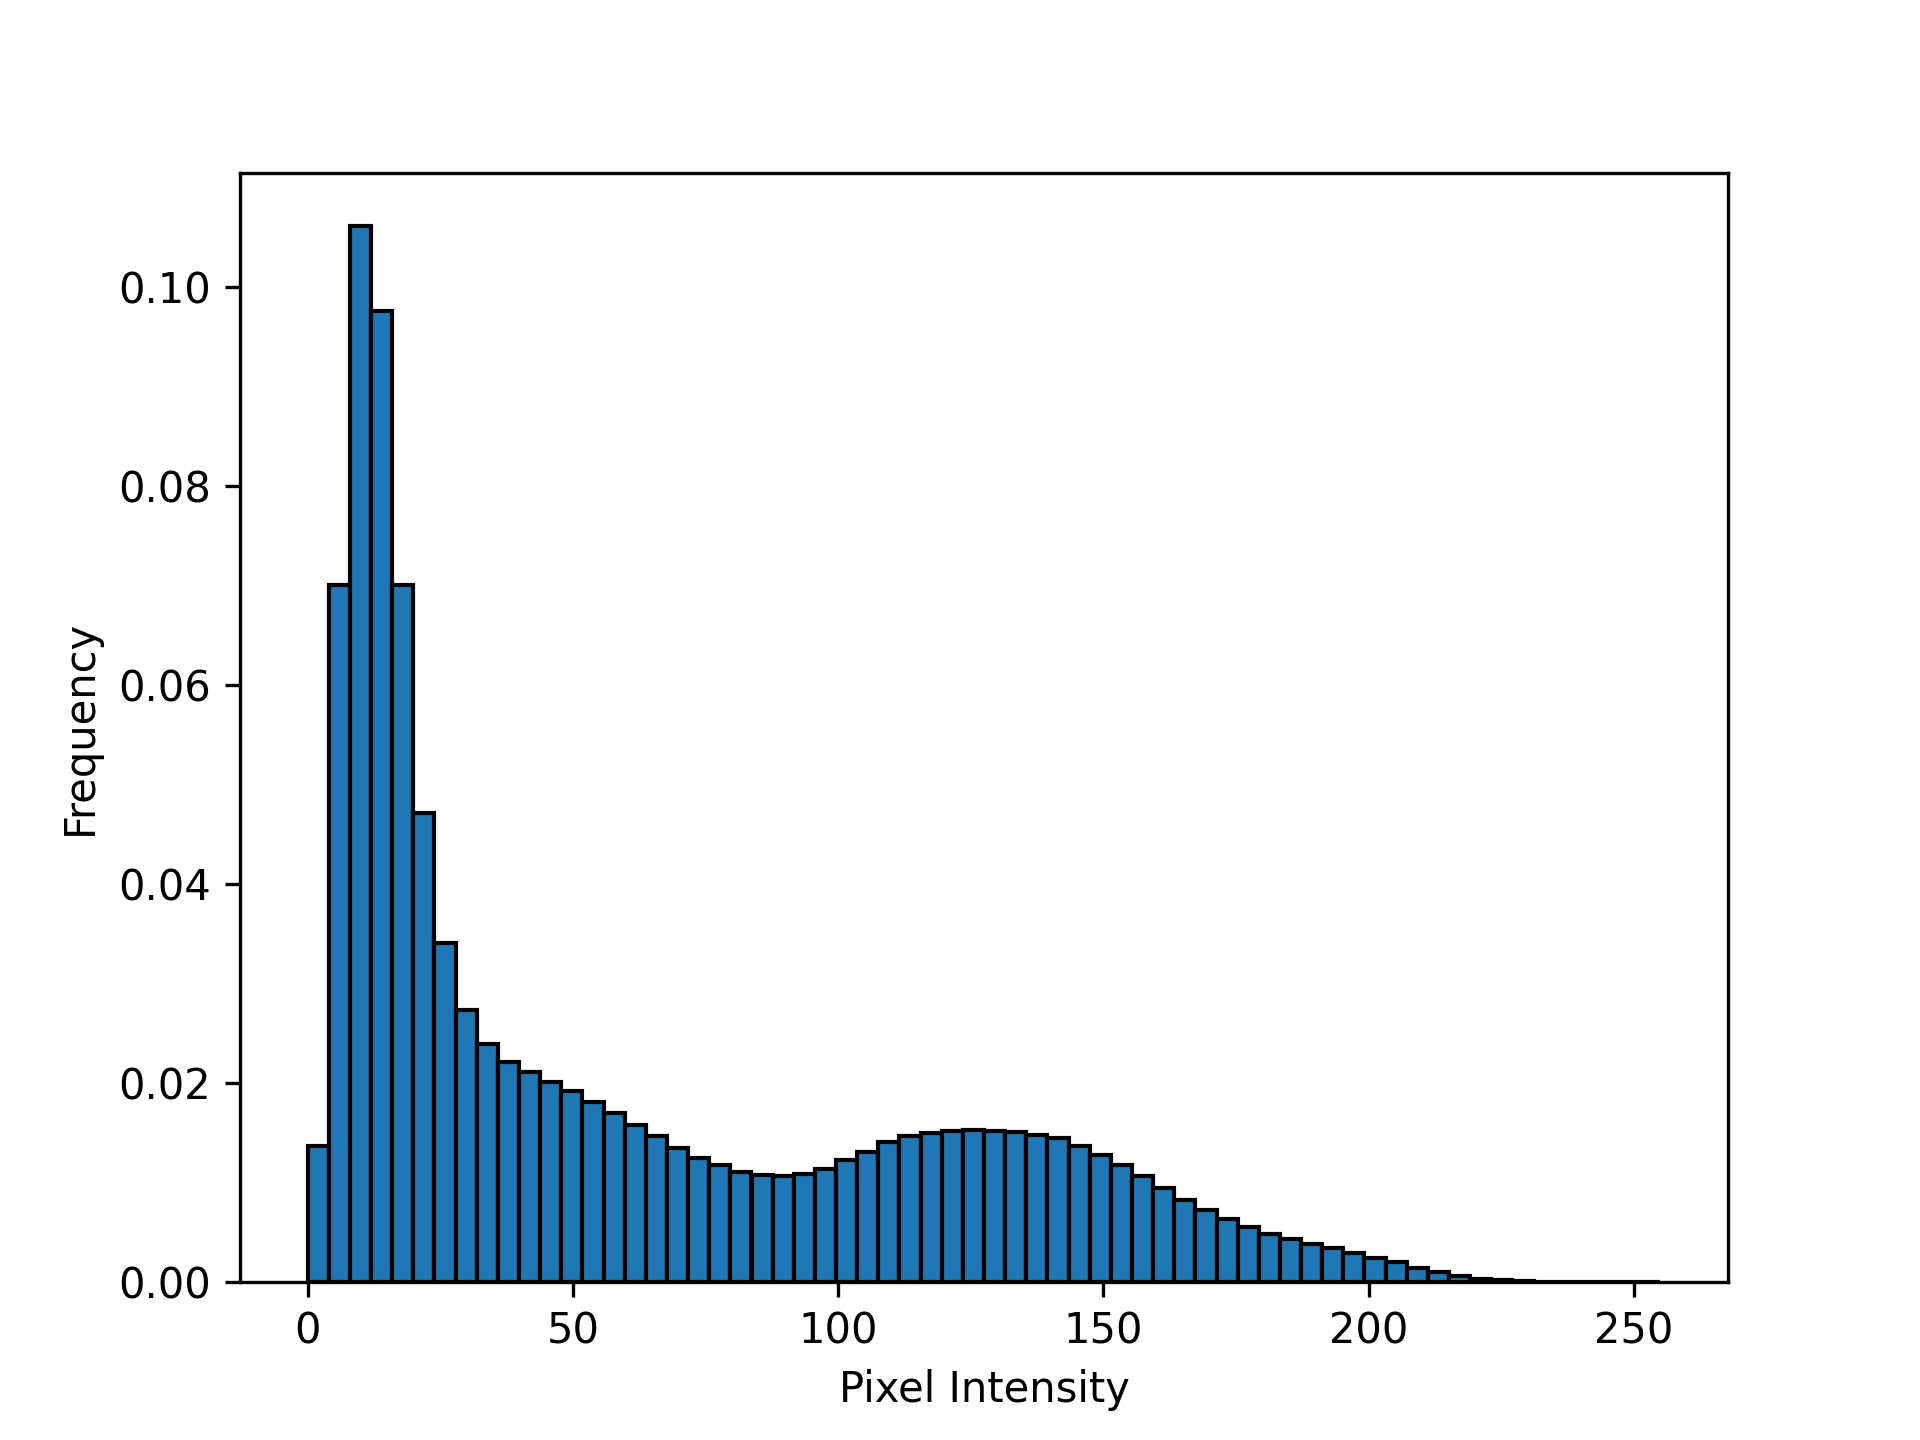
\includegraphics[width=0.8\textwidth]{img/normalized_histogram.png}
	\caption{Normalized histogram of the image}
	\label{fig:normalized_histogram}
\end{figure}

\begin{lstlisting}[language=Python, caption={Continuation of Listing \ref{lst:correlation}, to compute and plot the normalised histogram}]
# grayscale image for pixel intensities
img_gray = img[:, :, 0] * 0.2989 + img[:, :, 1] * 0.5870 + img[:, :, 2] * 0.1140
plt.imshow(img_gray, cmap="gray")

# histogram
h = np.zeros(256)
for i in range(img.shape[0]):
    for j in range(img.shape[1]):
        h[int(img_gray[i, j])] += 1
# normalized histogram
p = h / (img_gray.shape[0] * img_gray.shape[1])

# plot the normalized histogram
plt.figure()
_ = plt.hist(np.arange(256), weights=p, bins=64, edgecolor="black")
plt.xlabel("Pixel Intensity")
plt.ylabel("Frequency")
plt.savefig("normalized_histogram.png")
\end{lstlisting}
